% Preview of every new figure/table at NeurIPS text width (5.5in). Not for submission.
\documentclass[10pt]{article}
\usepackage[textwidth=5.5in,textheight=9in]{geometry}
\usepackage{newtxtext,newtxmath}
\usepackage{booktabs,graphicx,caption,float}
\captionsetup{font=small}
\graphicspath{{../figs/}}
\newcommand{\flamecl}{\textsc{FLAME-CL}}
\begin{document}
\section*{Figures}
\begin{figure}[H]\centering
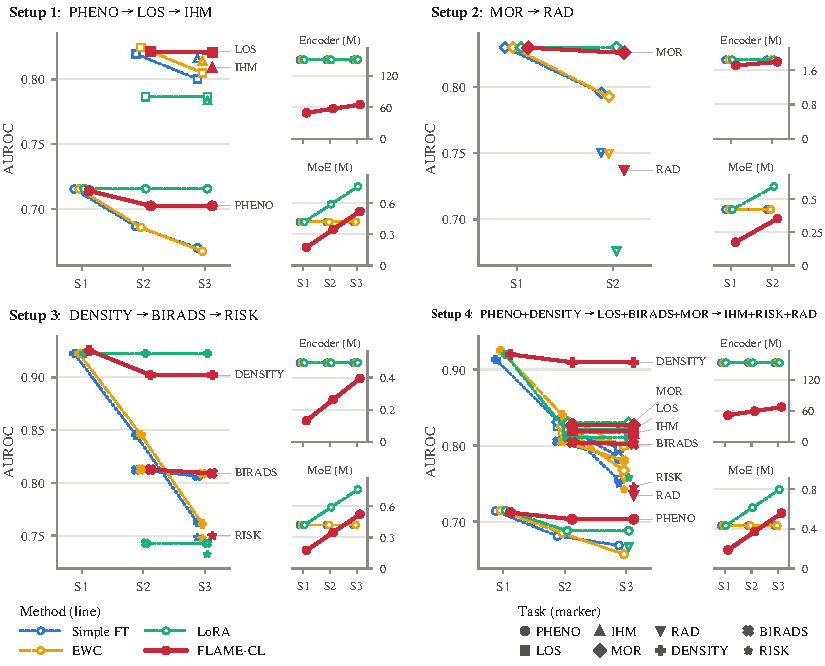
\includegraphics[width=\textwidth]{fig5_cl_trajectories_compact.pdf}
\caption{(Fig.~5 redraw, compact main-text version, about the height of the original.) Per-stage continual-learning trajectories for \textsc{Simple FT}, EWC, \textsc{LoRA} (MoE adapters) and \flamecl{} on the four task sequences (seed 42): AUROC of every task seen so far after each stage S$k$ (marker = task; colour and line style = method; \flamecl{} solid), with encoder and MoE parameters at inference. For \flamecl{} the value at a task's own stage is before rank-32 truncation. Numbers in Tab.~\ref{tab:cl-fig5-per-stage}; AUPRC in Fig.~10.}
\end{figure}
\begin{figure}[H]\centering
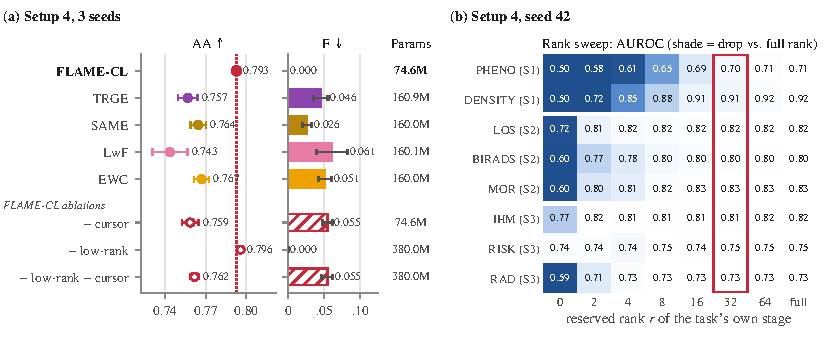
\includegraphics[width=\textwidth]{fig_cl_summary_tab3_tab4.pdf}
\caption{(Replaces Tabs.~3--4 on page 9.) (a) Setup 4, 3 timestamp seeds: average accuracy (AA, dot $\pm$ std), forgetting F (bar $\pm$ std) and parameters after three stages, for \flamecl{}, the baselines and the component ablations (hatched/hollow). (b) CL-phase rank sweep (Setup 4, seed 42): AUROC when the active component of a task's own stage is truncated to rank $r$, earlier stages frozen at rank 32; shade = drop relative to full rank; $r=32$ (default) outlined. Full numbers in Tabs.~14 and 16.}
\end{figure}
\begin{figure}[H]\centering
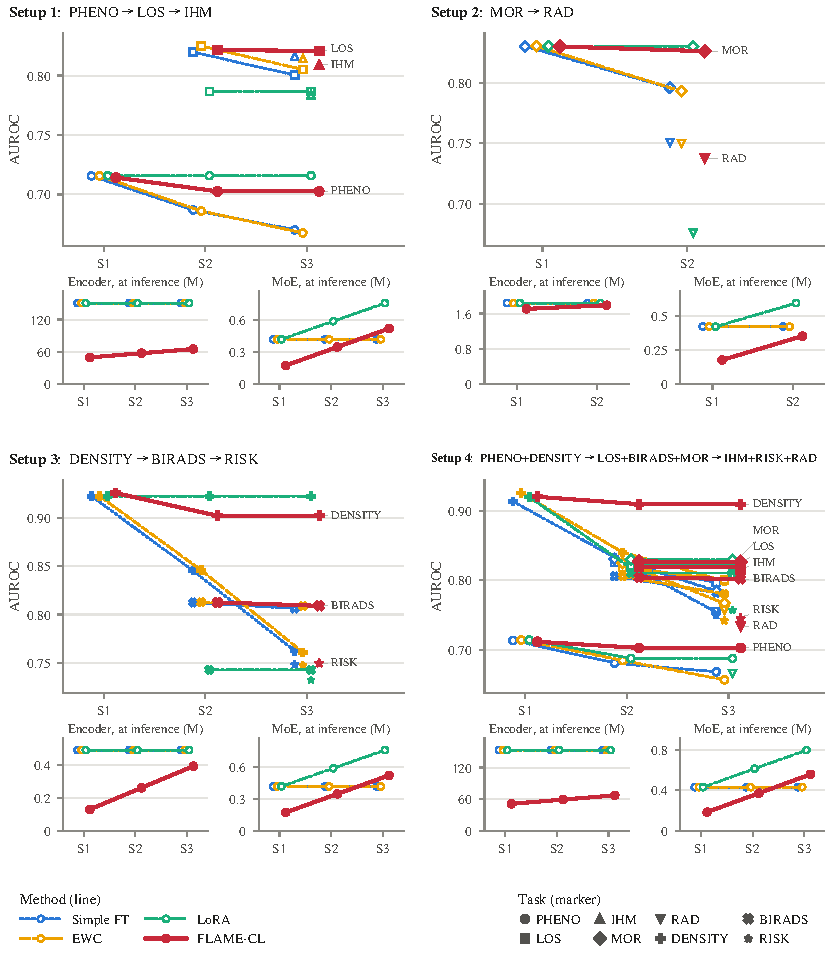
\includegraphics[width=\textwidth]{fig5_cl_trajectories.pdf}
\caption{(Fig.~5 redraw, full-size version for an appendix or if space allows.) Same content as the compact version, with the parameter panels below each AUROC panel.}
\label{fig:cl}\end{figure}
\begin{figure}[H]\centering
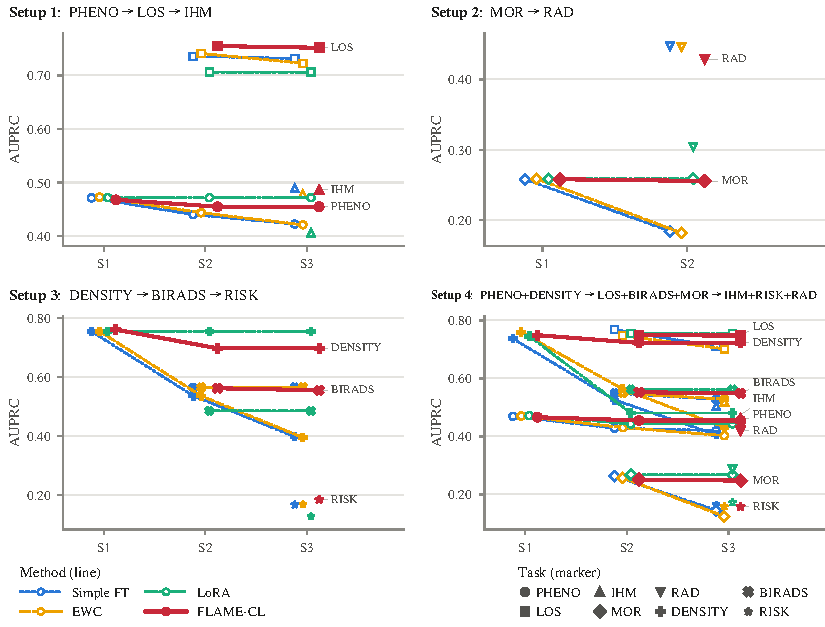
\includegraphics[width=\textwidth]{fig10_cl_auprc.pdf}
\caption{(Fig.~10 redraw) Per-stage AUPRC; methods and encoding as in Fig.~\ref{fig:cl}.}\end{figure}
\begin{figure}[H]\centering
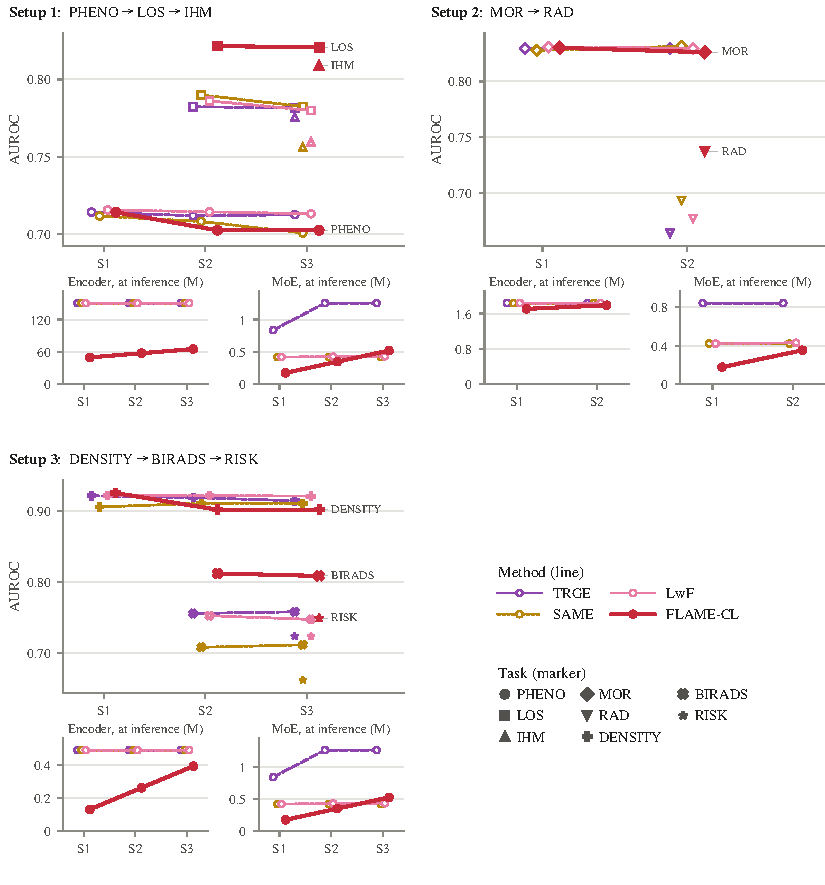
\includegraphics[width=\textwidth]{fig_cl_new_baselines_setups123.pdf}
\caption{(New, appendix) \flamecl{} against TRGE, SAME and L\textsc{w}F on Setups 1--3 (seed 42). Parameter panels show inference-time totals: the three baselines adapt only the MoE and keep the full encoder. Numbers in Tab.~\ref{tab:cl-new-baselines-s123}.}\end{figure}
\begin{figure}[H]\centering
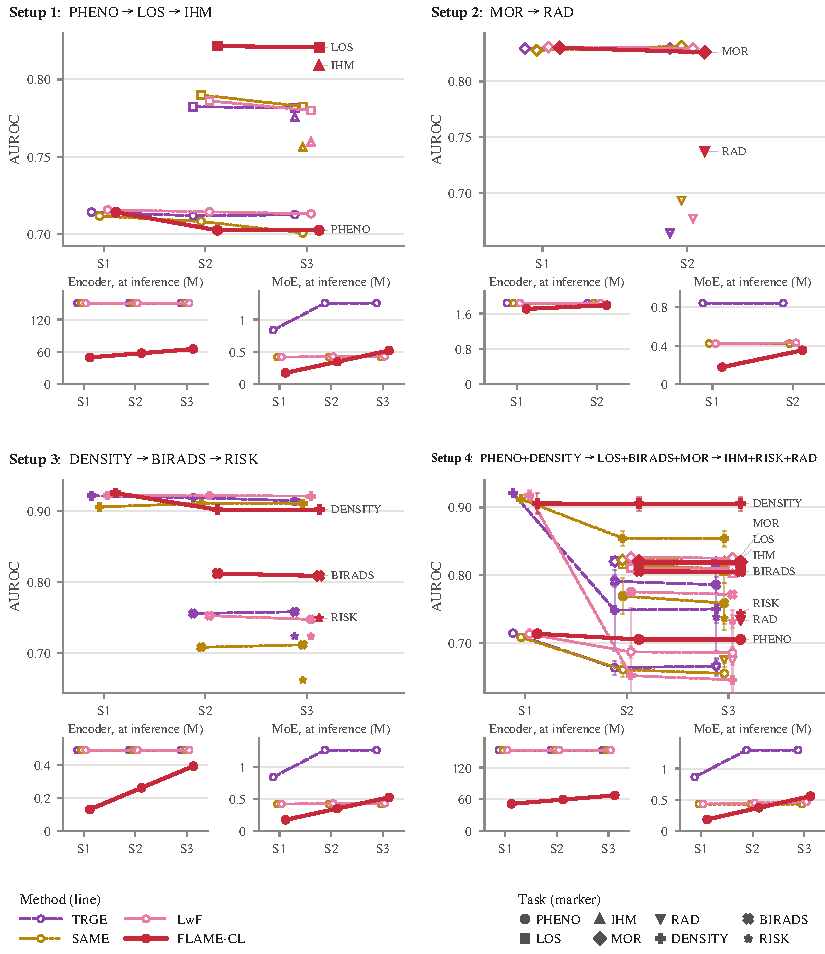
\includegraphics[width=\textwidth]{fig_cl_new_baselines.pdf}
\caption{(Alternative) Same as above with Setup 4 added (mean $\pm$ std over the three timestamp seeds of Tabs.~3, 13, 14).}\end{figure}
\begin{figure}[H]\centering
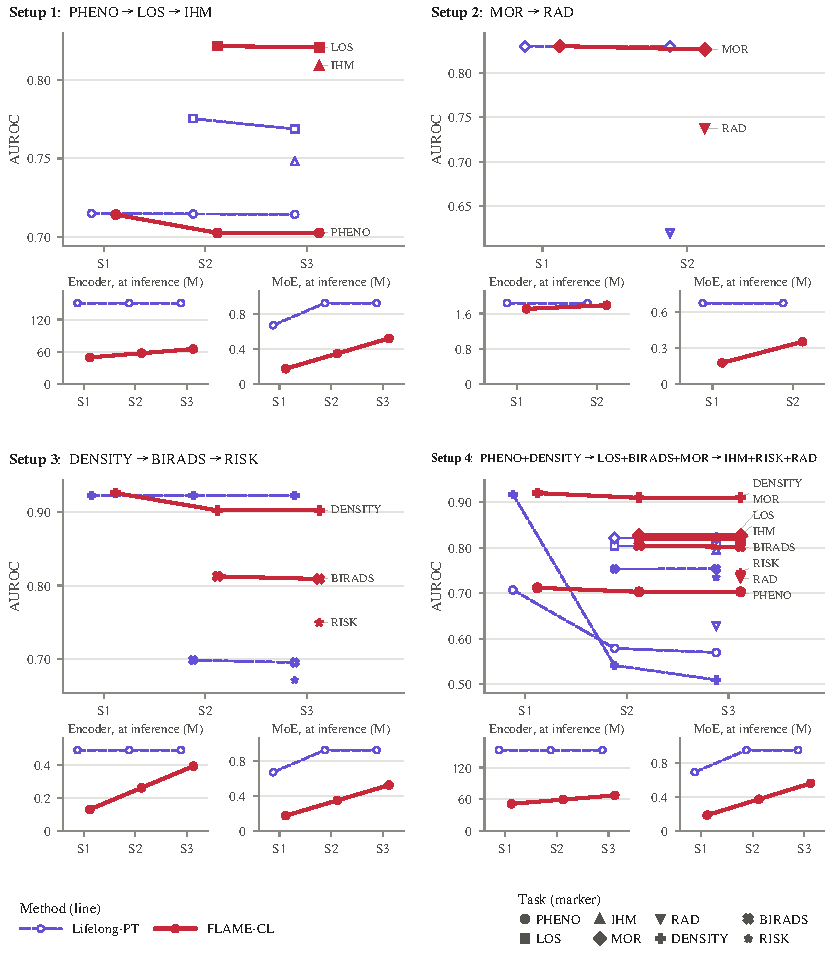
\includegraphics[width=\textwidth]{fig8_cl_vs_lifelong_pt.pdf}
\caption{(Fig.~8 redraw) \flamecl{} vs.\ Lifelong-PT, same runs as Fig.~\ref{fig:cl}; parameter panels are inference-time totals.}\end{figure}
\begin{figure}[H]\centering
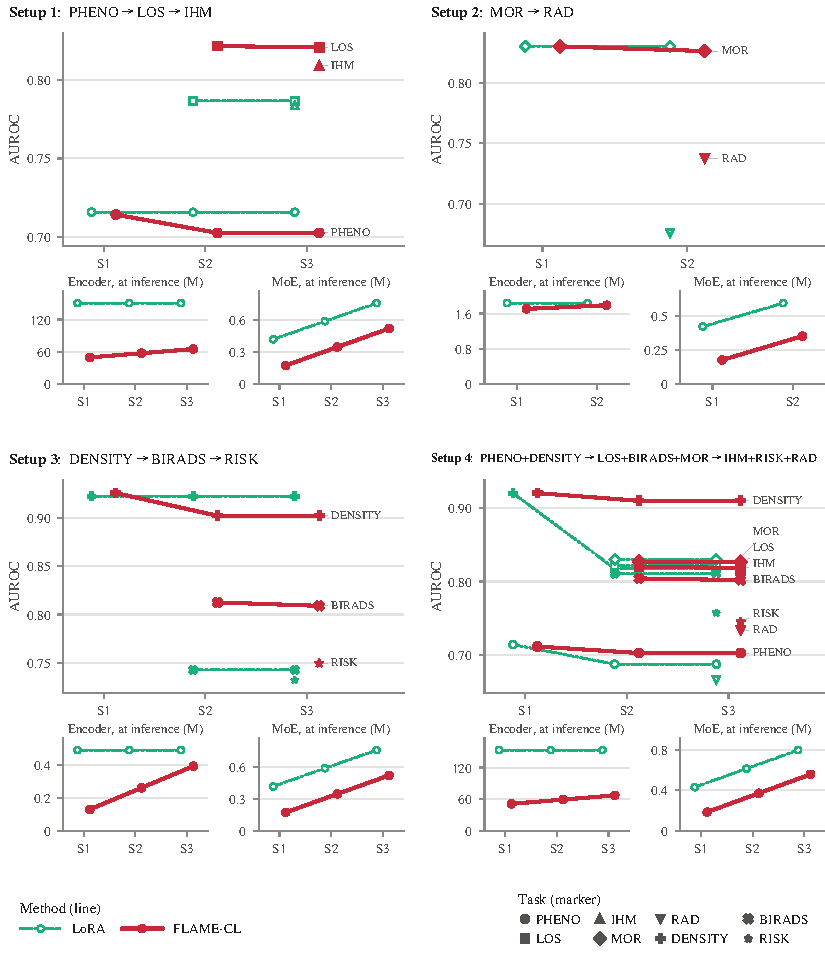
\includegraphics[width=\textwidth]{fig9_cl_vs_lora.pdf}
\caption{(Fig.~9 redraw) \flamecl{} vs.\ \textsc{LoRA} (MoE adapters); a subset of Fig.~\ref{fig:cl}, so it can be dropped.}\end{figure}
\begin{figure}[H]\centering
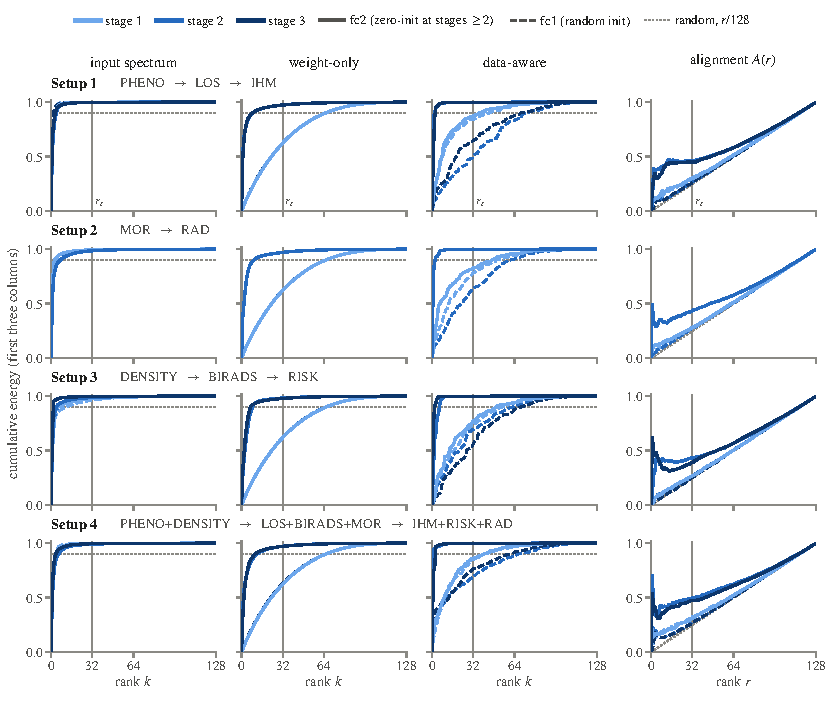
\includegraphics[width=\textwidth]{fig_cl_spectra_alignment.pdf}
\caption{(New, App.~D.4.3; path A, replaces Fig.~16.) Continual-stage spectra and singular-vector alignment for the four CL sequences (rows; \flamecl{}, seed 42): input spectrum, weight-only spectrum, data-aware energy, and $A(r)=\lVert V_r^\top Q_r\rVert_F^2/r$ (dotted: random, $r/128$). Median over the 5 experts; solid fc2 (zero-initialised at stages $\geq 2$), dashed fc1 (random init); colour = stage; vertical line $r_t=32$. Numbers in Tab.~\ref{tab:cl-spectra-alignment}.}\end{figure}
\begin{figure}[H]\centering
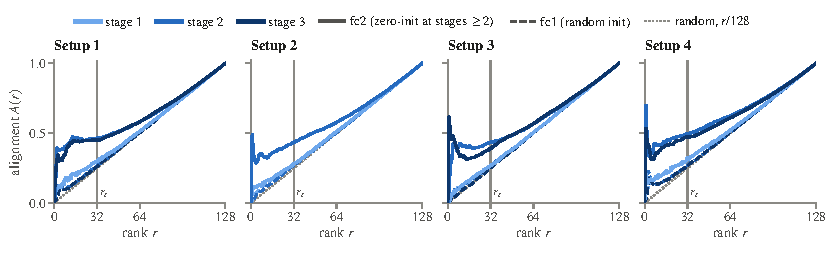
\includegraphics[width=\textwidth]{fig_cl_alignment.pdf}
\caption{(New, App.~D.4.3; path B, next to Fig.~16 extended with Setups 1--3.) Alignment column only.}\end{figure}
\begin{figure}[H]\centering
\includegraphics[width=\textwidth]{fig16_setup1_stage0.png}\\[2pt]
\includegraphics[width=\textwidth]{fig16_setup1_stage1.png}\\[2pt]
\includegraphics[width=\textwidth]{fig16_setup1_stage2.png}
\caption{(Path B) Fig.~16 format for Setup 1; Setups 2--3 are \texttt{figs/fig16\_setup\{2,3\}\_stage*.png}, layout in \texttt{tables/cl\_alignment\_snippets.tex}.}\end{figure}
\clearpage
\section*{Tables}
\begin{table}[t]
\centering
\footnotesize
\setlength{\tabcolsep}{3.5pt}
\caption{Per-stage numbers behind Fig.~\ref{fig:cl}: AUROC when first learned $\to$ after the final stage (seed 42). Stage-$K$ tasks report one value; drops of at least 0.02 in bold. For \textsc{FLAME-CL} the first value is before rank-32 truncation, so its deltas are the one-time truncation cost; F is measured against the deployed (post-truncation) model. Parameter rows give inference-time totals after the first $\to$ last stage; \textsc{LoRA} adapts only the MoE and keeps the full encoder.}
\label{tab:cl-fig5-per-stage}
\begin{tabular}{lcccc}
\toprule
Task (stage) & \textsc{Simple FT} & EWC & \textsc{LoRA} & \textsc{FLAME-CL} \\
\midrule
\multicolumn{5}{l}{\emph{Setup 1:} \textsc{Pheno} $\to$ \textsc{Los} $\to$ \textsc{Ihm}} \\
\addlinespace[1pt]
PHENO (s1) & 0.716 $\to$ \textbf{0.670} & 0.716 $\to$ \textbf{0.668} & 0.716 $\to$ 0.716 & 0.714 $\to$ 0.703 \\
LOS (s2) & 0.820 $\to$ 0.800 & 0.825 $\to$ 0.805 & 0.787 $\to$ 0.787 & 0.822 $\to$ 0.821 \\
IHM (s3) & 0.816 & 0.814 & 0.784 & 0.809 \\
\addlinespace[1pt]
AA $\uparrow$ & 0.762 & 0.762 & 0.762 & \textbf{0.777} \\
F $\downarrow$ & 0.032 & 0.034 & 0.000 & 0.000 \\
Enc.\ params, at inference (M) & 150.6 & 150.6 & 150.6 & 49.6$\to$65.1 \\
MoE params, at inference (M) & 0.42 & 0.42 & 0.42$\to$0.76 & 0.17$\to$0.52 \\
\midrule
\multicolumn{5}{l}{\emph{Setup 2:} \textsc{Mor} $\to$ \textsc{Rad}} \\
\addlinespace[1pt]
MOR (s1) & 0.830 $\to$ \textbf{0.796} & 0.830 $\to$ \textbf{0.793} & 0.830 $\to$ 0.830 & 0.830 $\to$ 0.826 \\
RAD (s2) & 0.751 & 0.750 & 0.676 & 0.737 \\
\addlinespace[1pt]
AA $\uparrow$ & 0.773 & 0.771 & 0.753 & \textbf{0.782} \\
F $\downarrow$ & 0.034 & 0.037 & 0.000 & 0.000 \\
Enc.\ params, at inference (M) & 1.84 & 1.84 & 1.84 & 1.71$\to$1.79 \\
MoE params, at inference (M) & 0.42 & 0.42 & 0.42$\to$0.59 & 0.18$\to$0.35 \\
\midrule
\multicolumn{5}{l}{\emph{Setup 3:} \textsc{Density} $\to$ \textsc{Birads} $\to$ \textsc{Risk}} \\
\addlinespace[1pt]
DENSITY (s1) & 0.923 $\to$ \textbf{0.762} & 0.923 $\to$ \textbf{0.761} & 0.923 $\to$ 0.923 & 0.926 $\to$ \textbf{0.902} \\
BIRADS (s2) & 0.812 $\to$ 0.806 & 0.813 $\to$ 0.809 & 0.743 $\to$ 0.743 & 0.813 $\to$ 0.809 \\
RISK (s3) & 0.748 & 0.748 & 0.732 & 0.750 \\
\addlinespace[1pt]
AA $\uparrow$ & 0.772 & 0.772 & 0.799 & \textbf{0.820} \\
F $\downarrow$ & 0.083 & 0.083 & 0.000 & 0.000 \\
Enc.\ params, at inference (M) & 0.49 & 0.49 & 0.49 & 0.13$\to$0.39 \\
MoE params, at inference (M) & 0.42 & 0.42 & 0.42$\to$0.76 & 0.17$\to$0.52 \\
\midrule
\multicolumn{5}{l}{\emph{Setup 4:} \{\textsc{Pheno}, \textsc{Density}\} $\to$ \{\textsc{Los}, \textsc{Birads}, \textsc{Mor}\} $\to$ \{\textsc{Ihm}, \textsc{Risk}, \textsc{Rad}\}} \\
\addlinespace[1pt]
PHENO (s1) & 0.714 $\to$ \textbf{0.669} & 0.714 $\to$ \textbf{0.657} & 0.714 $\to$ \textbf{0.688} & 0.712 $\to$ 0.703 \\
DENSITY (s1) & 0.913 $\to$ \textbf{0.754} & 0.925 $\to$ \textbf{0.799} & 0.920 $\to$ \textbf{0.818} & 0.920 $\to$ 0.909 \\
LOS (s2) & 0.825 $\to$ \textbf{0.797} & 0.819 $\to$ 0.800 & 0.822 $\to$ 0.822 & 0.820 $\to$ 0.819 \\
BIRADS (s2) & 0.806 $\to$ \textbf{0.782} & 0.806 $\to$ \textbf{0.780} & 0.810 $\to$ 0.810 & 0.804 $\to$ 0.802 \\
MOR (s2) & 0.831 $\to$ \textbf{0.785} & 0.825 $\to$ \textbf{0.767} & 0.830 $\to$ 0.830 & 0.827 $\to$ 0.827 \\
IHM (s3) & 0.823 & 0.824 & 0.808 & 0.815 \\
RISK (s3) & 0.750 & 0.742 & 0.758 & 0.745 \\
RAD (s3) & 0.755 & 0.757 & 0.667 & 0.734 \\
\addlinespace[1pt]
AA $\uparrow$ & 0.764 & 0.766 & 0.775 & \textbf{0.794} \\
F $\downarrow$ & 0.060 & 0.057 & 0.026 & 0.000 \\
Enc.\ params, at inference (M) & 153.0 & 153.0 & 153.0 & 51.4$\to$67.4 \\
MoE params, at inference (M) & 0.43 & 0.43 & 0.43$\to$0.80 & 0.19$\to$0.56 \\
\bottomrule
\end{tabular}
\end{table}

\begin{table}[t]
\centering
\footnotesize
\setlength{\tabcolsep}{3.5pt}
\caption{Setups 1--3: AUROC when first learned $\to$ after the final stage for \textsc{FLAME-CL} and the MoE-based / distillation baselines (seed 42; Setup 4 is in Tabs.~\ref{tab:cl-setup4-retention},~\ref{tab:cl-setup4-forgetting}). Drops of at least 0.02 in bold; F against the model deployed at the stage where each task was learned. Parameter rows give inference-time totals after the first $\to$ last stage: TRGE, SAME and L\textsc{w}F adapt only the MoE and keep the full encoder.}
\label{tab:cl-new-baselines-s123}
\begin{tabular}{lccccc}
\toprule
Task (stage) & \textsc{FLAME-CL} & TRGE & SAME & L\textsc{w}F & EWC \\
\midrule
\multicolumn{6}{l}{\emph{Setup 1:} \textsc{Pheno} $\to$ \textsc{Los} $\to$ \textsc{Ihm}} \\
\addlinespace[1pt]
PHENO (s1) & 0.714 $\to$ 0.703 & 0.714 $\to$ 0.713 & 0.712 $\to$ 0.701 & 0.716 $\to$ 0.713 & 0.716 $\to$ \textbf{0.668} \\
LOS (s2) & 0.822 $\to$ 0.821 & 0.782 $\to$ 0.782 & 0.790 $\to$ 0.782 & 0.786 $\to$ 0.780 & 0.825 $\to$ 0.805 \\
IHM (s3) & 0.809 & 0.776 & 0.756 & 0.760 & 0.814 \\
\addlinespace[1pt]
AA $\uparrow$ & \textbf{0.777} & 0.757 & 0.747 & 0.751 & 0.762 \\
F $\downarrow$ & 0.000 & 0.001 & 0.009 & 0.004 & 0.034 \\
Enc.\ params, at inference (M) & 49.6$\to$65.1 & 150.6 & 150.6 & 150.6 & 150.6 \\
MoE params, at inference (M) & 0.17$\to$0.52 & 0.84$\to$1.26 & 0.42 & 0.42$\to$0.43 & 0.42 \\
\midrule
\multicolumn{6}{l}{\emph{Setup 2:} \textsc{Mor} $\to$ \textsc{Rad}} \\
\addlinespace[1pt]
MOR (s1) & 0.830 $\to$ 0.826 & 0.830 $\to$ 0.829 & 0.828 $\to$ 0.832 & 0.831 $\to$ 0.830 & 0.830 $\to$ \textbf{0.793} \\
RAD (s2) & 0.737 & 0.665 & 0.694 & 0.678 & 0.750 \\
\addlinespace[1pt]
AA $\uparrow$ & \textbf{0.782} & 0.747 & 0.763 & 0.754 & 0.771 \\
F $\downarrow$ & 0.000 & 0.000 & 0.000 & 0.001 & 0.037 \\
Enc.\ params, at inference (M) & 1.71$\to$1.79 & 1.84 & 1.84 & 1.84 & 1.84 \\
MoE params, at inference (M) & 0.18$\to$0.35 & 0.84 & 0.42 & 0.42$\to$0.43 & 0.42 \\
\midrule
\multicolumn{6}{l}{\emph{Setup 3:} \textsc{Density} $\to$ \textsc{Birads} $\to$ \textsc{Risk}} \\
\addlinespace[1pt]
DENSITY (s1) & 0.926 $\to$ \textbf{0.902} & 0.922 $\to$ 0.915 & 0.906 $\to$ 0.911 & 0.923 $\to$ 0.921 & 0.923 $\to$ \textbf{0.761} \\
BIRADS (s2) & 0.813 $\to$ 0.809 & 0.756 $\to$ 0.759 & 0.708 $\to$ 0.712 & 0.753 $\to$ 0.748 & 0.813 $\to$ 0.809 \\
RISK (s3) & 0.750 & 0.724 & 0.663 & 0.724 & 0.748 \\
\addlinespace[1pt]
AA $\uparrow$ & \textbf{0.820} & 0.799 & 0.762 & 0.798 & 0.772 \\
F $\downarrow$ & 0.000 & 0.003 & 0.000 & 0.003 & 0.083 \\
Enc.\ params, at inference (M) & 0.13$\to$0.39 & 0.49 & 0.49 & 0.49 & 0.49 \\
MoE params, at inference (M) & 0.17$\to$0.52 & 0.84$\to$1.26 & 0.42 & 0.42$\to$0.43 & 0.42 \\
\bottomrule
\end{tabular}
\end{table}

\begin{table}[t]
\centering
\scriptsize
\setlength{\tabcolsep}{1.8pt}
\caption{Setup 4 per-task AUROC when first learned $\to$ after the final stage (3 timestamp-generated seeds, mean $\pm$ std). Stage-3 tasks are learned last and report one value. Drops of at least 0.02 in bold.}
\label{tab:cl-setup4-retention}
\begin{tabular}{lccccc}
\toprule
Task (stage) & \textsc{FLAME-CL} & TRGE & SAME & L\textsc{w}F & EWC \\
\midrule
PHENO (s1) & $0.71_{\pm 0.00}$ $\to$ $0.71_{\pm 0.00}$ & $0.71_{\pm 0.00}$ $\to$ $\mathbf{0.67}_{\pm 0.01}$ & $0.71_{\pm 0.00}$ $\to$ $\mathbf{0.65}_{\pm 0.01}$ & $0.71_{\pm 0.01}$ $\to$ $\mathbf{0.69}_{\pm 0.01}$ & $0.71_{\pm 0.00}$ $\to$ $\mathbf{0.67}_{\pm 0.00}$ \\
DENSITY (s1) & $0.91_{\pm 0.01}$ $\to$ $0.91_{\pm 0.01}$ & $0.92_{\pm 0.00}$ $\to$ $\mathbf{0.75}_{\pm 0.06}$ & $0.91_{\pm 0.01}$ $\to$ $\mathbf{0.85}_{\pm 0.01}$ & $0.92_{\pm 0.01}$ $\to$ $\mathbf{0.65}_{\pm 0.10}$ & $0.92_{\pm 0.01}$ $\to$ $\mathbf{0.78}_{\pm 0.05}$ \\
LOS (s2) & $0.82_{\pm 0.00}$ $\to$ $0.82_{\pm 0.00}$ & $0.82_{\pm 0.00}$ $\to$ $0.82_{\pm 0.00}$ & $0.82_{\pm 0.00}$ $\to$ $0.81_{\pm 0.01}$ & $0.81_{\pm 0.01}$ $\to$ $0.81_{\pm 0.00}$ & $0.82_{\pm 0.00}$ $\to$ $0.80_{\pm 0.01}$ \\
BIRADS (s2) & $0.81_{\pm 0.00}$ $\to$ $0.81_{\pm 0.00}$ & $0.79_{\pm 0.01}$ $\to$ $0.79_{\pm 0.01}$ & $0.77_{\pm 0.03}$ $\to$ $0.76_{\pm 0.03}$ & $0.78_{\pm 0.01}$ $\to$ $0.77_{\pm 0.00}$ & $0.80_{\pm 0.00}$ $\to$ $0.79_{\pm 0.01}$ \\
MOR (s2) & $0.82_{\pm 0.00}$ $\to$ $0.82_{\pm 0.00}$ & $0.82_{\pm 0.00}$ $\to$ $0.82_{\pm 0.00}$ & $0.82_{\pm 0.00}$ $\to$ $0.82_{\pm 0.00}$ & $0.83_{\pm 0.00}$ $\to$ $0.83_{\pm 0.00}$ & $0.82_{\pm 0.00}$ $\to$ $\mathbf{0.78}_{\pm 0.02}$ \\
IHM (s3) & $0.81_{\pm 0.01}$ & $0.81_{\pm 0.00}$ & $0.81_{\pm 0.02}$ & $0.80_{\pm 0.00}$ & $0.81_{\pm 0.00}$ \\
RISK (s3) & $0.74_{\pm 0.00}$ & $0.74_{\pm 0.01}$ & $0.74_{\pm 0.02}$ & $0.73_{\pm 0.01}$ & $0.75_{\pm 0.00}$ \\
RAD (s3) & $0.73_{\pm 0.00}$ & $0.66_{\pm 0.01}$ & $0.68_{\pm 0.00}$ & $0.67_{\pm 0.01}$ & $0.75_{\pm 0.00}$ \\
\bottomrule
\end{tabular}
\end{table}

\begin{table}[t]
\centering
\footnotesize
\setlength{\tabcolsep}{3pt}
\caption{Setup 4 per-task forgetting F and summary metrics (3 timestamp-generated seeds, mean $\pm$ std). F is measured against the model deployed at the stage where each task was learned (post-truncation for \textsc{FLAME-CL}).}
\label{tab:cl-setup4-forgetting}
\begin{tabular}{lccccc}
\toprule
 & \textsc{FLAME-CL} & TRGE & SAME & L\textsc{w}F & EWC \\
\midrule
F: PHENO (s1) & $0.000\pm0.000$ & $0.048\pm0.009$ & $0.054\pm0.007$ & $0.028\pm0.002$ & $0.043\pm0.005$ \\
F: DENSITY (s1) & $0.000\pm0.000$ & $0.171\pm0.061$ & $0.058\pm0.011$ & $0.272\pm0.109$ & $0.143\pm0.054$ \\
F: LOS (s2) & $0.000\pm0.000$ & $0.002\pm0.000$ & $0.006\pm0.005$ & $0.001\pm0.001$ & $0.020\pm0.011$ \\
F: BIRADS (s2) & $0.000\pm0.000$ & $0.005\pm0.004$ & $0.011\pm0.010$ & $0.004\pm0.002$ & $0.009\pm0.011$ \\
F: MOR (s2) & $0.000\pm0.000$ & $0.001\pm0.001$ & $0.003\pm0.002$ & $0.001\pm0.000$ & $0.041\pm0.021$ \\
\midrule
F (avg) $\downarrow$ & $0.000\pm0.000$ & $0.046\pm0.010$ & $0.026\pm0.007$ & $0.061\pm0.022$ & $0.051\pm0.009$ \\
BWT (avg) $\uparrow$ & $0.000\pm0.000$ & $-0.046\pm0.010$ & $-0.026\pm0.007$ & $-0.061\pm0.022$ & $-0.051\pm0.009$ \\
AA (8 tasks) $\uparrow$ & $0.793\pm0.002$ & $0.757\pm0.007$ & $0.764\pm0.006$ & $0.743\pm0.013$ & $0.767\pm0.006$ \\
\bottomrule
\end{tabular}
\end{table}

\begin{table}[t]
\centering
\footnotesize
\setlength{\tabcolsep}{4pt}
\caption{Per-task AUROC under the router-balancing loss weight sweep (joint nine-task training, $\lambda_{\mathrm{int}}=0.1$; mean $\pm$ std over seeds 42, 20492, 28411). $^\dagger$ default. Bold: best weight per task. Range: max $-$ min of the task mean across this sweep.}
\label{tab:aux-bal-per-task}
\begin{tabular}{llcccccc}
\toprule
 & & \multicolumn{5}{c}{$\lambda_{\mathrm{bal}}$} & \\
\cmidrule(lr){3-7}
Dataset & Task & 0 & 0.001 & 0.01$^\dagger$ & 0.1 & 1 & Range \\
\midrule
MIMIC-IV & 48-IHM & 0.801{\scriptsize$\pm$0.013} & 0.806{\scriptsize$\pm$0.009} & 0.809{\scriptsize$\pm$0.004} & 0.806{\scriptsize$\pm$0.007} & \textbf{0.815{\scriptsize$\pm$0.005}} & 0.013 \\
 & LOS & 0.812{\scriptsize$\pm$0.007} & 0.808{\scriptsize$\pm$0.003} & \textbf{0.817{\scriptsize$\pm$0.002}} & 0.812{\scriptsize$\pm$0.005} & 0.811{\scriptsize$\pm$0.007} & 0.009 \\
 & 25-PHENO & 0.715{\scriptsize$\pm$0.003} & \textbf{0.718{\scriptsize$\pm$0.001}} & 0.718{\scriptsize$\pm$0.001} & 0.716{\scriptsize$\pm$0.002} & 0.712{\scriptsize$\pm$0.001} & 0.006 \\
\addlinespace[2pt]
eICU & MOR & 0.838{\scriptsize$\pm$0.007} & 0.839{\scriptsize$\pm$0.007} & 0.839{\scriptsize$\pm$0.005} & 0.837{\scriptsize$\pm$0.002} & \textbf{0.839{\scriptsize$\pm$0.006}} & 0.003 \\
 & RAD & 0.759{\scriptsize$\pm$0.003} & \textbf{0.760{\scriptsize$\pm$0.002}} & 0.759{\scriptsize$\pm$0.001} & 0.754{\scriptsize$\pm$0.006} & 0.758{\scriptsize$\pm$0.005} & 0.006 \\
\addlinespace[2pt]
EMBED & BIRADS & \textbf{0.809{\scriptsize$\pm$0.004}} & 0.806{\scriptsize$\pm$0.001} & 0.804{\scriptsize$\pm$0.003} & 0.804{\scriptsize$\pm$0.003} & 0.803{\scriptsize$\pm$0.003} & 0.006 \\
 & RISK & 0.747{\scriptsize$\pm$0.004} & 0.752{\scriptsize$\pm$0.004} & 0.752{\scriptsize$\pm$0.006} & \textbf{0.753{\scriptsize$\pm$0.006}} & 0.750{\scriptsize$\pm$0.005} & 0.006 \\
 & DENSITY & 0.914{\scriptsize$\pm$0.012} & 0.914{\scriptsize$\pm$0.003} & 0.915{\scriptsize$\pm$0.003} & 0.910{\scriptsize$\pm$0.006} & \textbf{0.916{\scriptsize$\pm$0.001}} & 0.006 \\
\addlinespace[2pt]
ADNI & DIAG & 0.755{\scriptsize$\pm$0.033} & \textbf{0.788{\scriptsize$\pm$0.020}} & 0.771{\scriptsize$\pm$0.044} & 0.765{\scriptsize$\pm$0.026} & 0.751{\scriptsize$\pm$0.029} & 0.036 \\
\midrule
\multicolumn{2}{l}{Mean (9 tasks)} & 0.795{\scriptsize$\pm$0.001} & \textbf{0.799{\scriptsize$\pm$0.002}} & 0.798{\scriptsize$\pm$0.005} & 0.795{\scriptsize$\pm$0.003} & 0.795{\scriptsize$\pm$0.003} & 0.004 \\
\bottomrule
\end{tabular}
\end{table}

\begin{table}[t]
\centering
\footnotesize
\setlength{\tabcolsep}{4pt}
\caption{Per-task AUROC under the interaction loss weight sweep (joint nine-task training, $\lambda_{\mathrm{bal}}=0.01$; mean $\pm$ std over seeds 42, 20492, 28411). $^\dagger$ default. Bold: best weight per task. Range: max $-$ min of the task mean across this sweep.}
\label{tab:aux-int-per-task}
\begin{tabular}{llccccc}
\toprule
 & & \multicolumn{4}{c}{$\lambda_{\mathrm{int}}$} & \\
\cmidrule(lr){3-6}
Dataset & Task & 0 & 0.01 & 0.1$^\dagger$ & 1 & Range \\
\midrule
MIMIC-IV & 48-IHM & 0.806{\scriptsize$\pm$0.006} & 0.808{\scriptsize$\pm$0.004} & 0.809{\scriptsize$\pm$0.004} & \textbf{0.816{\scriptsize$\pm$0.006}} & 0.010 \\
 & LOS & 0.814{\scriptsize$\pm$0.008} & 0.808{\scriptsize$\pm$0.003} & 0.817{\scriptsize$\pm$0.002} & \textbf{0.817{\scriptsize$\pm$0.006}} & 0.009 \\
 & 25-PHENO & 0.713{\scriptsize$\pm$0.002} & \textbf{0.718{\scriptsize$\pm$0.001}} & 0.718{\scriptsize$\pm$0.001} & 0.712{\scriptsize$\pm$0.003} & 0.006 \\
\addlinespace[2pt]
eICU & MOR & 0.835{\scriptsize$\pm$0.005} & 0.839{\scriptsize$\pm$0.005} & 0.839{\scriptsize$\pm$0.005} & \textbf{0.840{\scriptsize$\pm$0.006}} & 0.005 \\
 & RAD & 0.757{\scriptsize$\pm$0.002} & 0.757{\scriptsize$\pm$0.006} & 0.759{\scriptsize$\pm$0.001} & \textbf{0.762{\scriptsize$\pm$0.004}} & 0.006 \\
\addlinespace[2pt]
EMBED & BIRADS & 0.804{\scriptsize$\pm$0.005} & 0.801{\scriptsize$\pm$0.004} & 0.804{\scriptsize$\pm$0.003} & \textbf{0.806{\scriptsize$\pm$0.002}} & 0.006 \\
 & RISK & 0.747{\scriptsize$\pm$0.004} & 0.749{\scriptsize$\pm$0.009} & \textbf{0.752{\scriptsize$\pm$0.006}} & 0.748{\scriptsize$\pm$0.001} & 0.005 \\
 & DENSITY & \textbf{0.917{\scriptsize$\pm$0.003}} & 0.910{\scriptsize$\pm$0.009} & 0.915{\scriptsize$\pm$0.003} & 0.915{\scriptsize$\pm$0.007} & 0.007 \\
\addlinespace[2pt]
ADNI & DIAG & 0.770{\scriptsize$\pm$0.027} & 0.762{\scriptsize$\pm$0.028} & \textbf{0.771{\scriptsize$\pm$0.044}} & 0.762{\scriptsize$\pm$0.031} & 0.009 \\
\midrule
\multicolumn{2}{l}{Mean (9 tasks)} & 0.796{\scriptsize$\pm$0.004} & 0.795{\scriptsize$\pm$0.002} & \textbf{0.798{\scriptsize$\pm$0.005}} & 0.798{\scriptsize$\pm$0.002} & 0.003 \\
\bottomrule
\end{tabular}
\end{table}

\begin{table}[t]
\centering
\footnotesize
\setlength{\tabcolsep}{4pt}
\caption{Rank correlations behind App.~\ref{app:robustness} (Setup 4 \textsc{FLAME-CL}, 31 (task, modality) pairs, 186 corrupted evaluations). Importance is the AUROC lost when the modality is removed; routing reaction is the Jensen--Shannon divergence of the gate distribution of a modality from its clean one. Per-task $p$-values are exact permutation tests ($n=3$--$5$ modalities).}
\label{tab:robustness-spearman}
\begin{tabular}{lccc}
\toprule
Pooled over all pairs & Spearman $\rho$ & $p$ & Pearson $r$ \\
\midrule
Routing JSD at 2$\times$ noise vs. importance & $+0.14$ & 0.44 & $-0.14$ \\
Routing JSD at 4$\times$ noise vs. importance & $+0.06$ & 0.75 & $-0.19$ \\
Routing JSD under shuffling vs. importance & $+0.12$ & 0.53 & $+0.27$ \\
Routing JSD at 2$\times$ noise vs. contribution share & $+0.13$ & 0.48 & $-0.21$ \\
Fusion contribution share vs. importance & $+0.73$ & $2.7\times10^{-6}$ & $+0.80$ \\
Fusion magnitude share vs. importance & $+0.53$ & $2.4\times10^{-3}$ & $+0.79$ \\
\bottomrule
\end{tabular}
\\[6pt]
\begin{tabular}{lcccccccc}
\toprule
Share vs.\ importance, per task & PHENO & DENSITY & LOS & BIRADS & MOR & IHM & RISK & RAD \\
\midrule
Modalities $n$ & 3 & 4 & 3 & 4 & 5 & 3 & 4 & 5 \\
Spearman $\rho$ & $+1.00$ & $+0.80$ & $+1.00$ & $+1.00$ & $+1.00$ & $+1.00$ & $+0.00$ & $+0.20$ \\
Exact $p$ & 0.33 & 0.33 & 0.33 & 0.08 & 0.02 & 0.33 & 1.00 & 0.78 \\
Smallest attainable $p$ & 0.33 & 0.08 & 0.33 & 0.08 & 0.02 & 0.33 & 0.08 & 0.02 \\
\bottomrule
\end{tabular}
\end{table}

\begin{table}[t]
\centering
\scriptsize
\setlength{\tabcolsep}{3.2pt}
\caption{Continual-phase spectra and singular-vector alignment of the active component of each stage (FLAME-CL, seed 42), median over the 5 experts, reported as fc2\,/\,fc1. $r_{90}$: rank at 90\% cumulative energy (ambient 128). Kept: data-aware energy inside the top-32 singular directions, i.e.\ what survives the $r_t{=}32$ truncation. $A(r)=\lVert V_r^\top Q_r\rVert_F^2/r$ between the top-$r$ right singular vectors of the component and the top-$r$ eigenvectors of its routed-input second moment; random subspaces give $r/128$ (0.125 at $r{=}16$, 0.25 at $r{=}32$). fc2 is zero-initialised at stages $\geq$2; fc1, and both sublayers at stage 1, start from random init.}
\label{tab:cl-spectra-alignment}
\begin{tabular}{@{}llccccc@{}}
\toprule
 & & \multicolumn{3}{c}{$r_{90}$ (fc2\,/\,fc1)} & Kept at $r_t{=}32$ & $A(16)$ \\
\cmidrule(lr){3-5}
Setup & Stage & input & weight-only & data-aware & data-aware & (random 0.125) \\
\midrule
1 & 1: PHENO & 4\,/\,4 & 65\,/\,66 & 37\,/\,45 & 0.87\,/\,0.84 & 0.21\,/\,0.20 \\
 & 2: LOS & 5\,/\,3 & 9\,/\,65 & 2\,/\,74 & 1.00\,/\,0.51 & 0.46\,/\,0.14 \\
 & 3: IHM & 4\,/\,2 & 9\,/\,65 & 3\,/\,69 & 1.00\,/\,0.65 & 0.44\,/\,0.15 \\
\addlinespace[2pt]
2 & 1: MOR & 3\,/\,7 & 66\,/\,66 & 47\,/\,50 & 0.83\,/\,0.78 & 0.17\,/\,0.17 \\
 & 2: RAD & 8\,/\,7 & 10\,/\,66 & 3\,/\,62 & 1.00\,/\,0.64 & 0.36\,/\,0.15 \\
\addlinespace[2pt]
3 & 1: DENSITY & 6\,/\,12 & 66\,/\,65 & 50\,/\,55 & 0.77\,/\,0.74 & 0.16\,/\,0.15 \\
 & 2: BIRADS & 5\,/\,6 & 9\,/\,66 & 6\,/\,62 & 1.00\,/\,0.69 & 0.41\,/\,0.16 \\
 & 3: RISK & 2\,/\,2 & 7\,/\,66 & 2\,/\,69 & 1.00\,/\,0.56 & 0.32\,/\,0.12 \\
\addlinespace[2pt]
4 & 1: PHENO+DENSITY & 4\,/\,4 & 66\,/\,66 & 41\,/\,41 & 0.86\,/\,0.85 & 0.21\,/\,0.23 \\
 & 2: LOS+BIRADS+MOR & 7\,/\,5 & 12\,/\,66 & 1\,/\,68 & 1.00\,/\,0.69 & 0.44\,/\,0.16 \\
 & 3: IHM+RISK+RAD & 4\,/\,5 & 11\,/\,65 & 3\,/\,61 & 1.00\,/\,0.76 & 0.41\,/\,0.16 \\
\bottomrule
\end{tabular}
\end{table}

\paragraph{D.6 drop-in text.}% Drop-in wording for App. D.6 (numbers from make_robustness_stats.py)
% "Routers do not downweight unreliable modalities; the fusion head does." paragraph:
Routing does react to corruption, with the Jensen--Shannon divergence from the clean gate rising with the noise level on every task, but that reaction is uncorrelated with the modality's importance (Spearman $\rho=+0.14$, $p=0.44$, $n=31$ (task, modality) pairs). Reliability weighting instead resides in the fusion head: the learned share of each modality in the fusion logit correlates with its measured importance (the AUROC drop on removal) at $\rho=+0.73$ ($p=2.7\times10^{-6}$, $n=31$), and per task at $\rho=+1$ on 5 of 8 tasks (Tab.~\ref{tab:robustness-spearman}).

\end{document}
